\chapter{Dasar Teori}
\label{chap:dasar teori}

Sebelum bisa membuat Twitter bot untuk mencari jalur transportasi publik, berikut diberikan beberapa definisi yang berkaitan dengan pembuatan Twitter bot. Bab ini akan menjelaskan Twitter, Twitter API, KIRI, KIRI API, dan Twitter4j.

\section{Twitter}
\label{sec:twitter}

Twitter adalah layanan yang memungkinkan pengguna untuk mengirim pesan menggunakan 140 karakter atau kurang. Pesan tersebut dapat diadaptasikan melalui teks, aplikasi \textit{mobile}, atau web. (referensi dari buku Sams teach yourself the twitter api) Berikut ini adalah daftar istilah umum pada Twitter:

Twitter adalah salah satu layanan jejaring sosial online yang memungkinkan pengguna memposting pesan berbasis teks hingga 140 karakter (referensi dari buku The Twitter Book).
\begin{itemize}
	\item Tweet 
	
	Posting pada Twitter disebut sebagai \textit{tweet}. \textit{Tweet} ini akan meneruskan pesan singkat yang ditujukan ke semua \textit{follower} suatu akun\footnote{Dusty Reagan, \textit{Twitter Application Development For Dummies}, Wiley, 2010, page 7}. Contohnya adalah seorang akun @kviniink ingin menuliskan bahwa hari ini cuaca cerah, maka @kviniink akan men-tweet 'Hari ini cerah yah..' Tweet juga bisa menyertakan link ke video, foto, atau media lain di internet selain teks biasa. URL link teks termasuk ke dalam 140 batas karakter, namun URL tersebut akan menghabisnya tempat/space dari keterbatasan karakter tweet. Oleh karena itu URL akan dibuat versi singkatnya, contoh saat pengguna memasukkan link 'http://www.chacha.com/gallery/7253/15-movies-that-make-guys-cry', maka akan dibuat menjadi 'bit.ly/1uRi8vV'.
	\item Follow
	
	Follow adalah satu istilah dalam Twitter yang bertujuan untuk mengikuti aktivitas \textit{tweet} suatu akun. Following adalah ketika sebuah akun mengikuti akun orang lain, dan Follower adalah ketika sebuah akun melakukan aksi follow kepada akun anda.
	\item Reply 
	
	Reply adalah cara seseorang untuk dapat memberi rujukan kepada akun Twitter yang lainnya atau lebih dikenal dengan nama \textit{mention}\footnote{Dusty Reagan, \textit{Twitter Application Development For Dummies}, Wiley, 2010, page 9}. Sebagai contoh, diketahui akun bernama @kviniink mem-\textit{follow} @infobdg untuk mengetahui perkembangan apa saja yang tejadi di kota Bandung. Lalu akun @kviniink ingin bertanya tentang info mall yang ramai di Bandung, maka akun @kviniink membuat \textit{mention tweet} yang berisikan "@infobdg Halo saya ingin bertanya apa saja mall yang sedang ramai di Bandung yah?".
	\item Retweet
	
	Retweet ini merupakan salah satu yang paling penting dari Twitter(referensi the twitter book halaman 47). Retweet ini berguna ketika pengguna menemukan tweet menarik dan berbagi tweet tersebut dengan follower akun tersebut (\textit{follower}). Retweet ini juga secara tidak langsung mengatakan bahwa "saya menghormati anda dan pesan yang anda buat".
	
	\item Hashtag
	
	Sebuah fitur yang diciptakan oleh Twitter untuk membantu pencarian kata kunci dan penandaan suatu diskusi.
	
	\item Direct Message(DM)
	
	Direct message digunakan untuk mengirim pesan yang bersifat private antara dua orang. Orang yang mengirim direct message ini hanya bisa untuk orang yang mengikuti akun tersebut.
	\item Timeline
	
	Timeline adalah sekumpulan tweet-tweet dari semua orang yang anda follow lalu akan ditampilkan di halaman utama.
\end{itemize}


\section{Twitter API}
Twitter API adalah aplikasi pihak ketiga yang memungkinkan \textit{programmer} melakukan manipulasi dan pengolahan data di Twitter. Twitter API tidak seperti API pada umumnya karena Twitter memaparkan hampir semuanya termasuk \textit{setup account} dan informasi kostumisasi\cite{Twitter}. Ini adalah salah satu bentuk pendekatan dari Twitter yang berfokus pada jaringan dan memungkinkan developer memiliki hak untuk berpikir 'out of the box' untuk membuat aplikasi yang mereka inginkan. Tetapi tetap akan terjadi keterbatasan yang dimiliki Twitter API, yaitu :
\begin{itemize}
	\item Hanya bisa men-update 1000 per harinya, baik melalui handphone, website, API, dan sebagainya.
	\item Total pesan hanya bisa sebanyak 250 per harinya, pada setiap dan semua perangkat.
	\item 150 permintaan API per jam.
	\item OAuth diijinkan 350 permintaan per jam.
\end{itemize}

\subsection{Search API}

Twitter Search API memungkinkan melakukan pencarian terhadap tweet baru ataupun tweet populer. Tetapi Twitter Search API ini bukan fitur yang tersedia pada Twitter itu sendiri. API ini difokuskan kepada relefansi, bukan terhadap kelengkapan data. Ini berarti bahwa beberapa Tweet dan pengguna akan hilang dari hasil pencarian.

\paragraph{Bagaimana cara membuat sebuah query}
Cara berbaik dalam membuat sebuah query dan melakukan percobaan yang valid dan mengembalikan tweet yang sesuai dengan yang dilakukan pada twitter.com/search. URL yang ditampilkan pada browser akan berisi sintaks query yang sesuai agar dapat digunakan kempali pada API endpoint. Berikut adalah contohnya:

\begin{enumerate}
	\item Melakukan pencarian untuk tweet yang direferensikan kepada akun @twitterapi. Pertama kita harus melakukan pencarian pada twitter.com/search.
	\item Lakukan pengecekan dan salin URL yang ditampilkan. Sebagai contoh didapatkan URL seperti ini, https://twitter.com/search?q=\%40twitterapi
	\item Ganti "https://twitter.com/search" dengan "https://api.twitter.com/1.1/search/tweets.json" dan akan didapatkan "https://api.twitter.com/1.1/search/tweets.json?q=\%40twitterapi"
	\item Eksekusi URL tersebut untuk melakukan pencarian di dalam API.
\end{enumerate}

API v1.1 mewajibkan bahwa request harus diotentifikasi. Perlu diingat juga bahwa hasil pencarian yang dilakukan di twitter.com dapat menghasilkan hasil yang sudah sangat lama, sedangkan Search API hanya melayani tweet dari seminggu terakhir.

\begin{table}[h]
\begin{tabular}{ll}
Operator                   & Finds tweets                                                             \\
watching now               & containing both "watching" and "now". This is the default operator.       \\
"happy hour"               & containing the exact phrase "happy hour".                                 \\
love OR hate               & containing either "love" or "hate" (or both).                             \\
beer -root                 & containing "beer" but not "root".                                         \\
\#haiku                    & ontaining the hashtag "haiku".                                            \\
from:alexiskold            & sent from person "alexiskold".                                            \\
to:techcrunch              & sent to person "techcrunch".                                              \\
@mashable                  & referencing person "mashable".                                            \\
superhero since:2010-12-27 & containing "superhero" and sent since date "2010-12-27" (year-month-day). \\
ftw until:2010-12-27       & containing "ftw" and sent before the date "2010-12-27".                   \\
movie -scary :)            & containing "movie", but not "scary", and with a positive attitude.        \\
flight :(                  & containing "flight" and with a negative attitude.                         \\
traffic ?                  & containing "traffic" and asking a question.                               \\
hilarious filter:links     & containing "hilarious" and linking to URL.                                \\
news source:twitterfeed    & containing "news" and entered via TwitterFeed                            
\end{tabular}
\end{table}

Dipastikan bahwa melakukan pengkodean URL terhadap query terlebih dahulu sebelum melakukan request. Tabel berikut memberikan contoh mapping dari search query ke query pengkodean URL.

\begin{table}[h]
\begin{tabular}{ll}
Search query     & URL encoded query                 \\
\#haiku \#poetry & \%23haiku+\%23poetry              \\
"happy hour" :)  & \%22happy\%20hour\%22\%20\%3A\%29
\end{tabular}
\end{table}

\paragraph{Additional parameters}
Terdapat parameter tambahan yang dipergunakan untuk hasil pencarian yang lebih baik. Berikut adalah penjelasan dari parameter tambahan tersebut :

\begin{itemize}
	\item \textbf{\textit{Result Type}}. Seperti hasil yang terdapat pada twitter.com/search, parameter result\_type memungkinkan hasil pencarian akan berdasarkan tweet yang paling baru atau tweet yang paling poluler atau bahkan gabungan dari keduanya.
	\item \textit{\textbf{Geolocatization}}. Pencarian tempat tidak tersedia pada API, tetapi ada beberapa cara yang tepat untuk membatasi query dengan cara menggunakan parameter geocode lalu mementukan "latitude, longitude, radius". Contohnya adalah "37.781157,-122.398720,1mi". Ketika pencarian lokasi pencarian API pertama akan mencoba menemukan tweet yang memiliki latitude yang sudah dimasukan kedalam query geocode, jika tidak berhasil maka API akan mencoba menemukan tweet yang dibuat oleh pengguna yang lokasi profilenya terdapat pada latitude tersebut. Artinya adalah hasil pencarian mungkin menerima tweet yang tidak mencakup informasi latidute atau longitude.
	\item \textit{\textbf{Language}}. Bahasa dapat dijadikan parameter untuk mencari tweet yang sesuai dengan bahasa tersebut.
	\item \textbf{\textit{Iterating in a result set}}. Parameter seperti count, until, since\_id, max\_id memungkinkan untuk mengkontrol bagaimana iterasi melalui hasil pencarian.
\end{itemize}

\paragraph{Rate limits}
User pada saat ini diwakilkan oleh \textit{access tokens} yang dapat membuat 180 \textit{request} per 15 menit. Tetapi kita bisa membuat 450 request per 15 menit dengan cara menggunakan \textit{application-only authentication} atas nama sendiri tanpa konteks pengguna.

\paragraph{Contoh Pencarian}
Ketika anda mengikuti suatu acara yang sedang berlangsung, anda tertarik untuk mencarinya dengan melihat tweet yang paling baru dan menggunakan hastag dari acara tersebut, maka langkah-langkah yang dilakukan adalah:
\begin{itemize}
	\item Anda ingin mencari tweet yang paling baru dengan menggunakan hastag \#superbowl
	\item Maka search URL akan seperti ini:
	https://api.twitter.com/1.1/search/tweets.json?q=\%23superbowl\&result\_type=recent
\end{itemize}

Ketika anda ingin mengetahui tweet yang datang dari suatu lokasi dengan bahasa yang spesifik, maka langkah-langkah yang dilakukan adalah:
\begin{itemize}
	\item Anda ingin mencari tweet yang paling baru dalam Bahasa Portugal, yang lokasinya dekat Maracanã soccer stadium yang terletak di Rio de Janeiro.
	\item Maka search URL akan seperti ini:
	\vtop{\hbox{\strut https://api.twitter.com/1.1/search/tweets.json?}\hbox{\strut q=\&geocode=-22.912214,-43.230182,1km\&lang=pt\&result\_type=recent }}
	%%%https://api.twitter.com/1.1/search/tweets.json?q=\&geocode=-22.912214,-43.230182,1km\&lang=pt\&result\_type=recent
	
Ketika anda ingin mencari tweet yang sedang poluler dari spesifik user dan tweet tersebut terdapat sebuah hashtag tertentu:
\begin{itemize}
	\item Anda ingin mencari tweet yang poluler yang berasal dari @kviniink yang terdapat hashtag \#nasa.
	\item Maka search URL akan seperti ini:
	https://api.twitter.com/1.1/search/tweets.json?q=from\%3Akviniink\%20\%23nasa\&result\_type=popular
\end{itemize}
\end{itemize}

\subsection{Streaming API}
Streaming API adalah contoh \textit{real-time} API. API ini ditujukan bagi para pengembang dengan kebutuhan data yang intensif. Contohnya jika mencari cara untuk membangun sebuah data produk data-mining atau tertarik dalam analisis penelitian. Streaming API memungkinkan melacak kata kunci yang ditentukan dalam jumlah besar dan melakukan suatu aksi (seperti tweet) secara langsung atau \textit{real-time}.

Twitter menawarkan beberapa endpoint streaming, disesuaikan dengan kasus yang terjadi. 
\begin{itemize}
	\item Public stream
	
	Steaming data publik yang mengalir melalui Twitter. Dipergunakan untuk mengikuti sebuah akun atau topik tertentu. Selain itu juga public stream digunakan untuk data mining.
	\item User Stream
	
	Single-user streams, mengandung hampir semua data yang berhubungan dengan satu user tertentu.
	
	\item Site Stream
	
	Versi dari multi-user stream. Site stream harus terhubung dengan server yang terkoneksi dengan twitter atas nama banyak pengguna.
\end{itemize}


\subsection{Public Streams}
Stream ini menawarkan sampel data publik yang mengalir melalui Twitter. Ketika aplikasi membuat sambungan ke streaming endpoint, aplikasi akan menyampaikan umpan Tweet tanpa perlu khawatir akan keterbatasan rate limit.

\paragraph{Endpoints}
\begin{itemize}
	\item POST statuses / filter
	\item GET statuses / sample
	\item GET statuses / firehose
\end{itemize}

\paragraph{POST statuses/filter}
POST filter ini mengembalikan status publik yang sesuai dengan satu atau lebih predikat yang telah di filter. \textit{Multiple parameter} memungkinkan klien untuk menggunakan koneksi tunggal untuk ke Streaming API. Antara GET dan POST \textit{request} keduanya didukung tetapi GET \textit{request} yang memiliki parameter yang terlalu banyak mungkin akan ditolak karena URL yang terlalu panjang. Gunakanlah POST request untuk menghindari URL yang panjang.
Track, follow, dan lokasi harus dipertimbangkan untuk dapat digabungkan dengan operator OR. track=foo\&follow=1234 ini mengembalikan tweet yang memiliki kata "foo" atau dibuat oleh user 1234.
Hal ini memungkinkan akses hingga 400 kata kunci, 5000 \textit{follow users}, dan 250.1-360 derajat kotak lokasi.

\paragraph{Resource Information}
\begin{table}[h]
\begin{tabular}{|l|l|}
Response formats         & JSON                    \\
Requires authentication? & Ya (hanya \textit{user context}) \\
Rate limited?            & Ya                    
\end{tabular}
\end{table}


\paragraph{Parameter}
Perlu diperhatikan bahwa salah satu parameter (follow, location, atau track) harus diisi secara spesifik.

\begin{table}[h]
\begin{tabular}{ll}
follow          & Tanda koma memisahkan list user ID, hal ini menunjukkan pengguna untuk kembali ke status untuk stream. \\
track           & Kata pencarian untuk track. Fase kata kunci dipisahkan oleh tanda koma.                \\
locations       & Menentukan lokasi yang dilacak.                                                    \\
delimited       & Menentukan apakah pesan harus dibatasi limitnya.                                         \\
stall\_warnings & Menentukan apakah pesan warning harus dikirim atau tidak.                                         
\end{tabular}
\end{table}


\paragraph{GET statuses/sample}
Mengembalikan \textit{random} sampel dari semua status public. Tweet akan dikembalikan dengan cara seperti biasa, jadi jika terdapat dua client yang terhubung dengan \textit{endpoint} ini, maka mereka akan melihat Tweet yang sama.

\paragraph{Resource Information}
\begin{table}[h]
\begin{tabular}{|l|l|}
Response formats         & JSON                    \\
Requires authentication? & Ya (hanya \textit{user context}) \\
Rate limited?            & Ya                    
\end{tabular}
\end{table}


\paragraph{Parameter}

\begin{table}[h]
\begin{tabular}{ll}
delimited          & Menentukan apakah pesan harus dibatasi limitnya. \\
stall\_warning           & Menentukan apakah pesan warning harus dikirim atau tidak.                \\            
\end{tabular}
\end{table}


\paragraph{GET statuses/firehose}
Mengembalikan semua status public. Beberapa aplikasi membutuhan akses ini. Teknik ini diolah secara kreatif dengan cara menggabungkan sumber informasi yang ada dengan berbagai sumber lainnya maka dapat memuaskan pengguna.

\paragraph{Resource Information}
\begin{table}[h]
\begin{tabular}{|l|l|}
Response formats         & JSON                    \\
Requires authentication? & Ya (hanya \textit{user context}) \\
Rate limited?            & Ya                    
\end{tabular}
\end{table}


\paragraph{Parameter}

\begin{table}[h]
\begin{tabular}{ll}
count & Kumpulan pesan untuk dijadikan bahan materi \\
delimited          & Menentukan apakah pesan harus dibatasi limitnya. \\
stall\_warning           & Menentukan apakah pesan warning harus dikirim atau tidak.                \\            
\end{tabular}
\end{table}


\paragraph{Menggunakan Streaming API}
Proses menggunakan Streaming API adalah dengan cara menghubungkan endpoint yang sudah tercantum di atas dengan parameter yang sudah di list kepada streaming endpoint dan juga request parameter streaming API. Proses pengembalian data oleh streaming API dilakukan dengan cara mengikuti petunjuk dalam pengolahan data streaming.

\paragraph{Koneksi}
Setiap akun hanya dapat membuat satu koneksi yang terbuhung dengan \textit{public endpoint} dan jika melakukan koneksi ke public stream lebih dari satu kali dengan menggunakan akun yang sama akan menyebabkan koneksi terlama akan putus. Klien yang membuat koneksi secara berlebihan baik berhasil ataupun tidak maka IP mereka otomatis akan di \textit{banned}.

%User Streams
\subsection{User Streams}
User Stream memberikan aliran(\textit{stream}) data dan event yang spesific untuk pengguna yang sudah diotentifikasi. User Stream tidak dimaksudkan untuk koneksi server ke server, Jika anda perlu membuat koneksi atas nama beberapa user dari mesin yang sama maka lebih baik menggunakan site stream.

\paragraph{Endpoints}
\begin{itemize}
	\item GET user
\end{itemize}
\paragraph{Resource Information}
\begin{table}[h]
\begin{tabular}{|l|l|}
Response formats         & JSON                    \\
Requires authentication? & Ya (hanya user context) \\
Rate limited?            & Ya                    
\end{tabular}
\end{table}

\paragraph{Parameter}
\begin{table}[h]
\begin{tabular}{|l|l|}
delimited              & Menentukan apakah pesan harus dibatasi limitnya.																																					\\
stall\_warnings        & Menentukan apakah pesan warning harus dikirim atau tidak.                                                                        \\
with                   & Menentukan apakah pesan informasi harus dikembalikan untuk user yang sudah diotentifikasi atau dikirim juga kepada akun yang difollow oleh akun yang sudah diotentifikasi tersebut.\\
replies                & Menentukan apakah harus mengembalikan @replies.                                                                             \\
follow                 & Termasuk tweet public tambahan dari daftar yang disediakan ID pengguna.														\\
track                  & Termasuk tweet tambahan yang cocok dengan kata kunci tertentu.     \\
locations              & Termasuk tweet tambahan yang termasuk dalam batasan lokasi tertentu.                                                      \\
stringify\_friend\_ids & Mengirim list teman yang diterdiri dari array of integer dan array of string.                          
\end{tabular}
\end{table}

\paragraph{Koneksi}
Meminimalkan jumlah koneksi suatu aplikasi untuk membuat user stream. Setiap akun Twitter terbatas hanya untuk beberapa koneksi user streams per aplikasi OAuth, terlepas dari IP. Setelah mencapai batasnya maka koneksi tertua atau terlama akan diberhentikan secara otomatis. Akun login dari beberapa instansi dari aplikasi AOuth yang sama akan mengalami siklus koneksi yaitu akan dihubungan dan diputuskan satu sama lain.

Sebuah aplikasi harus dapat mengatasi HTTP 420 error code yang memberitahukan bahwa suatu akun sudah terlalu sering login. Oleh karena itu user yang seperti itu akan secara otomatis di \textit{banned} dari User Stream untuk tingkat login yang berlebihan. Untuk memulihkan akses streaming user harus menutup aplikasi tambahan yang ada, mungkin berjalan di perangkat atau device yang berbeda.

Perhatikan bahwa setiap aplikasi memiliki alokasinya masing-masing, sehingga login dari aplikasi pertama tidak akan mempengaruhi applikasi ke dua begitu juga sebaliknya. Tetapi menjalankan terlalu banyak salinan aplikasi pertama maupun ke dua akan menimbulkan masalah. Perhatikan juga bahwa jumlah koneksi yang serentak per alamat IP masih terbatas terlepas dari aplikasi yang ada.

%OAuth
\subsection{OAuth}
\label{sec:oauth}
Dengan semakin berkembangnya website, semakin banyak situs yang bergantung pada layanan distribusi dan \textit{cloud computing}. Contohnya adalah menggunakan jejaring sosial dengan menggunakan akun media sosial lainnya seperti Google untuk mencari teman-teman yang sudah tersimpan pada kontak Google. Atau bisa juga menggunakan pihak ketiga yang memanfaatkan API dari beberapa layanan.

OAuth menyediakan suatu metode bagi pengguna untuk memberi akses pihak ketiga untuk \textit{resources} (sumber daya) mereka tanpa berbagi password mereka.Cara ini juga memberikan cara untuk memberikan akses yang terbatas(dalam satu lingkup atau durasi) Sebagai contoh, seorang pengguna web dapat memberikan layanan percetakan(client) untuk mengakses foto pribadinya yang disimpan di layanan berbagi foto(server) tanpa harus memberikan username dan passwordnya. Ia akan mengotentikasi langsung dengan layanan berbagi foto tersebut yang mengeluarkan layanan percetakan.

Dalam model otentikasi client-server tradisional, klian menggunakan kredensial untuk mengakses \textit{recources hosted} oleh server. Di dalam model OAuth, klien (bukan pemilik resource, tetapi bertindak atas namanya) meminta akses ke \textit{resource} yang dikenalkan oleh pemilik \textit{resource} namun diselenggarakan oleh server.

Agar klien dapat mengakses \textit{resource}, pertama-tama ia harus mendapatkan izin dari si pemilik \textit{resource}. Izin ini dinyatakan dalam bentuk token dan mencocokan \textit{shared-secret}. Tujuan dari token ini adalah untuk membuat pemilik \textit{resource} untuk berbagi kepercayaan kepada klien. Berbeda dengan kepercayaan pemilik \textit{resource}. Token dapat dikeluarkan dalam ruang lingkup terbatas, durasi yang terbatas, dan akan dicabut secara independen. Reverensi(http://hueniverse.com/oauth/guide/intro/)

Twitter OAuth yang diberikan memiliki fitur
\begin{itemize}
	\item \textit{Secure}
	
	Pengguna tidak harus berbagi password mereka dengan aplikasi pihak ketiga untuk meningkatkan keamanan akun.
	\item \textit{Standard}
	
	Contoh code yang diberikan sudah kompatibel dengan implementasi Twitter OAuth.
\end{itemize}

\textit{API v1.1's Authentication Model}
Otentifikasi model baru terdapat dalam dua bentuk, dan keduanya masih memanfaatkan OAuth 1.0A


\textit{Application-user authentication}
\textit{Application-user authentication} adalah bentuk paling umum dari otentikasi \textit{resource} dalam pelaksanaan OAuth 1.0A Twitter sampai saat ini. Permintaan anda menandatangani baik untuk mengidentifikasi identitas aplikasi anda yang akan menyertakan izin untuk diberikan kepada pengguna. Hal ini bertujuan untuk dapat membuat panggilan API atas nama anda yang diwakili oleh akses token.

\textit{Application-only authentication}
\textit{Application-only authentication} adalah bentuk dari otentifikasi dimana aplikasi anda membuat \textit{API request} atas nama aplikasi itu sendiri tanpa adanya konteks dari pengguna. Pemanggilan API masih terbatas dalam setiap \textit{API method} .


\subsubsection{Application-only authentication}
Twitter menawarkan aplikasi yang mampu mengeluarkan permintaan otentifikasi atas nama aplikasi itu sendiri. Dengan menggunakan \textit{Application-only authentication} anda tidak mempunyai konteks dari otentikafikasi pengguna dan ini berarti setiap request API untuk endpoint akan membutuhkan konteks user, seperti memposting tweet tidak akan bekerja. Aplikasi yang akan di dapat adalah: 

\begin{itemize}
	\item Melihat timeline
	\item Mengakses following dan follower dari suatu akun
	\item Mencari dalam tweet
	\item mengambil informasi dari akun manapun
\end{itemize}


Tetapi \textit{application-only authentication} tidak bisa melakukan :

\begin{itemize}
	\item Posting tweet
	\item Melakukan koneksi dengan \textbf{Streaming endpoint}
	\item Mencari akun seseorang
	\item Menggunakan geo endpoint
	\item Mengakses DM
\end{itemize}

\paragraph{\textit{Auth Flow}}
Langkah-langkah dari \textit{application-only auth} terdiri dari beberapa langkah yaitu :
Sebuah aplkasi dikodekan berdasarkan \textit{consumer key} dan \textit{secret} ke dalam satu set khusus yang dikodekan secara kredensial.
Aplikasi membuat \textit{request} ke POST OAuth2/\textit{token endpoint} untuk merubah kredensial tersebut untuk \textit{token bearer}.
Ketika mengakses REST API, aplikasi menggunakan \textit{token bearer} untuk otentifikasi.
Kerena tidak ada kebutuhan duntuk menandatangani \textit{request}, pendekatan ini lebih sederhana dari model standar OAuth 1.0a

\begin{figure}
	\centering
		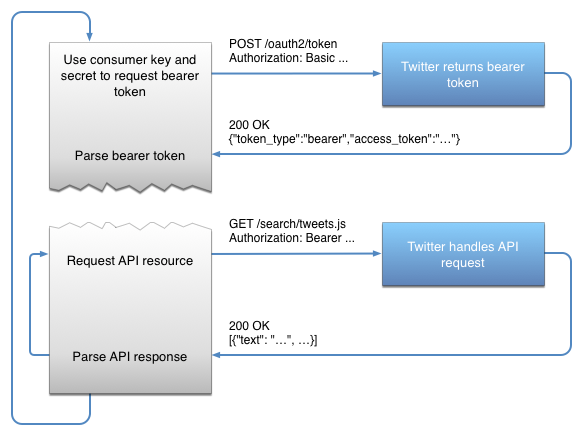
\includegraphics[width=1.00\textwidth]{C:/Users/Kvin/git/Skripsi/doc/DokumenSkripsi/Gambar/flow application-only authentication.png}
	\caption{flow application-only authentication}
	\label{fig:flow application-only authentication}
\end{figure}


\paragraph{Tentang Application-only Authentication}
Token adalah \textit{password}. Perlu diingat bahwa \textit{consumer key} dan \textit{secret, bearer token credential}, dan \textit{the bearer token} itu sendiri memberikan akses untuk membuat permintaan atas nama aplikasi itu sendiri. Point-point ini harus dianggap sensitif layaknya \textit{password} dan tidak boleh dibagikan atau didistribusikan kepada pihak yang tidak dipercaya atau tidak berkepentingan

SSL benar-benar dibutuhkan karena ini adalah cara otentifikasi yang aman. Oleh karena itu semua \textit{request} (baik untuk mendapatkan atau menggunakan token) harus menggunakan endpoint HTTPS, yang juga merupakan syarat untuk menggunakan API v1.1.

Tidak ada konteks pengguna. Ketika mengeluarkan permintaan menggunakan application-only auth, tidak ada konsep \textit{'current-user'}. Karena itu endpoint seperti POST status / update tidak akan berfungsi dengan \textit{application-only auth}.

\textit{Rate limiting}. \textit{Request} yang dibuat atas nama pengguna tidak akan menguras ketersediaan \textit{rate limit} dan \textit{request} tidak akan menguras batas penggunaan \textbf{limit} dalam \textit{user-based auth}.


\subsubsection{3-legged authorization}
Cara kerja dari \textit{3-legged authorization} adalah dengan memberikan aplikasi yang anda buat untuk mengambil \textit{access token} dengan cara melakukan \textit{redirect} user dengan Twitter dan memberikan mereka sebuah otorisasi dari aplikasi yang anda buat. Cara kerja ini hampir identik dengan cara kerja yang dijelaskan pada implementasi \textit{Sign in} dengan Twitter, hanya saja terdapat dua pengecualian yaitu:

\begin{itemize}
	\item \textit{GET oauth endpoint} digunakan sebagai pengganti GET oauth
	\item User akan selalu diminta untuk mengotorisasi akses ke aplikasi anda, bahkan jika akses sebelumnya telah diberikan
\end{itemize}

Beginilah ilustrasi interaksi \textit{sign in} dengan menggunakan \textit{following flowchart}

\begin{figure}[hp]
	\centering
		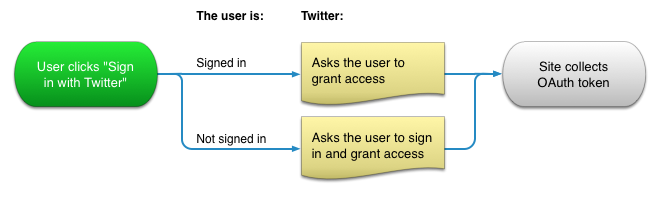
\includegraphics[width=1.00\textwidth]{C:/Users/Kvin/git/Skripsi/doc/DokumenSkripsi/Gambar/sign-in-flow3-3legged.png}
	\caption{Ilustrasi sign in}
	\label{fig:sign-in-flow3-3legged}
\end{figure}

\paragraph{PIN-based authorization}
cara kerja dari PIN-based authorization ini ditujukan untuk aplikasi yang tidak bisa mengakses atau menanamkan \textit{web browser} untuk mengarahkan user kepada \textit{authorization endpoint}. Contohnya adalah aplikasi yang bersifat \textit{command-line}, \textit{embedded systems}, \textit{game} konsol, dan beberapa jenis aplikasi \textit{mobile}.


Implementasi

Implementasi \textit{PIN-based} ini memiliki cara kerja yang sama seperti \textit{3-legged authorization}, perbedaannya terletak pada nilai dari \textit{oauth\_callback} yang harus di set menjadi \textit{oob} saat proses pemanggilan \textit{POST oauth atau request\_token}.

Setelah applikasi anda telah mendapatkan \textit{GET oauth/authenticate} atau \textit{GET oauth/authorize URL}, tampilkan URL kepada user agar mereka dapat menggunakan \textit{web browser} untuk mengakses Twitter.

Ketika \textit{callback oob} diminta dan user pengunjungi Twitter, user tidak akan dipindahkan secara otomatis ke aplikasi setelah menyetujui akses. Sebaliknya, mereka akan melihat PIN code, dengan instruksi untuk kembali ke aplikasi dan memasukkan nilai dari PIN code tersebut.

\begin{figure}[htbp]
	\centering
		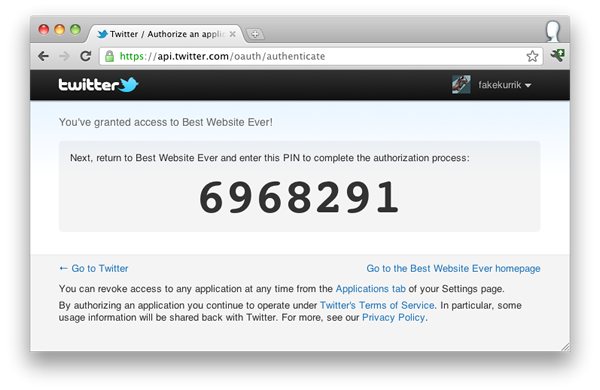
\includegraphics{C:/Users/Kvin/git/Skripsi/doc/DokumenSkripsi/Gambar/pin.png}
	\label{fig:pin}
\end{figure}

Aplikasi anda harus memungkinkan user untuk memasukkan \textit{PIN code} ini untuk menyelesaikan flow tersebut. Nilai dari \textit{PIN code} harus lolos sebagai oauth\_verifier untuk \textit{POST oauth/access\_token request}. semua request akan berjalan normal kedepannya.


%\section{KIRI}
%\label{sec:kiri}
%KIRI adalah sebuah situs atau \textit{website} yang memberi panduan tentang jalur transportasi publik. Alasan KIRI dapat berdiri adalah karenanya global warming, kemacetan, harga bensin yang semakin mahal. Ketiga alasan tersebut yang menjadi masalah sekarang ini, dan semua itu dapat diatasi dengan menaiki transportasi publik. 

%Peran dari KIRI ini adalah memberitahukan seseorang jalur transportasi publik dari satu tempat ke tempat yang dituju. Adapula format yang harus diisi dalam melakukan pencarian ini yaitu
%\begin{enumerate}
%	\item kota,
%	\item tempat awal,
%	\item tempat tujuan.
%\end{enumerate}

\subsection{KIRI API}
KIRI API adalah aplikasi pihak ketiga yang memungkinkan \textit{programmer} mendapatkan data tentang info jalur transportasi publik. KIRI API dapat diakses dengan beberapa cara. Semua \textit{request} harus berisikan API key, yang dapat diambil melalui KIRI API \textit{Management Dashboard}. Berikut adalah spesifikasi dari KIRI API

\begin{itemize}
	\item Routing Web Service
	\item Search Place Web Service
	\item Nearest Transports Web Service
\end{itemize}

\subsubsection{Routing Web Service}
Routing Web Service adalah salah satu KIRI API yang digunakan untuk mendapatkan langkah perjalanan dari lokasi asal menuju lokasi tujuan.

Berikut ini adalah parameter request yang diperlukan:

\begin{tabular}{ |l|l|l| }
	\hline
	Parameter & Valid values & Description \\ \hline \hline
  version & 2 & \vtop{\hbox{\strut Memberitahukan bahwa layanan yang dipakai} \hbox{\strut adalah protokol versi 2}} \\ \hline
  mode & "findroute" & Mengintruksikan layanan untuk mencari rute \\ \hline
  locale & "en" or "id" & Respon bahasa yang digunakan \\ \hline
	start & lat,lng (both are decimal values) & Titik awal \textit{Latitude} dan \textit{longitude} \\ \hline
  finish & lat,lng (both are decimal values) & Titik akhir \textit{Latitude} dan \textit{longitude}  \\ \hline
  presentation & "mobile" or "desktop" & \vtop{\hbox{\strut Menentukan tipe presentasi untuk hasil keluaran.}\hbox{\strut Contoh, jika tipe presentasi "mobile", }\hbox{\strut maka link "tel:" akan ditambahkan di hasil.}} \\ \hline
	apikey & 16-digit hexadecimals & API key yang digunakan \\ \hline
\end{tabular}

\begin{lstlisting} [caption= code \textit{respond} pencarian rute]
{ 
    "status": "ok" or "error" 
    "routingresults": [ 
        {
            "steps": [
                [
                    "walk" or "none" or others,
                    "walk" or vehicle_id or "none",
                    ["lat_1,lon_1", "lan_2,lon_2", ... "lat_n,lon_n"],
                    "human readable description, dependant on locale",
                    URL for ticket booking or null (future)
                ],
                [
                    "walk" or "none" or others,
                    "walk" or vehicle_id or "none",
                    ["lat_1,lon_1", "lan_2,lon_2", ... "lat_n,lon_n"],
                    "human readable description, dependant on locale",
                    URL for ticket booking or null (future)
                ]
            ],
            "traveltime": any text string, null if and only if route is not found.
        } ,
        {
            "steps": [ ... ],
            "traveltime": "..."
        } ,
        {
            "steps": [ ... ],
            "traveltime": "..."
        } ,
        ...     
    ]
}
\end{lstlisting}

Ketika pencarian route berhasil yaitu dengan memberitahukan bahwa status "ok" seperti pada baris 2, maka server juga harus memberikan hasil dari rute, yang berisikan langkah-langkah yang disimpan di dalam array. Berikut ini adalah keterangan dari array tersebut:

\begin{itemize}
	\item Indeks 0 (baris ke) berisikan "walk" atau "none" atau "others". Arti dari "walk" adalah jalan kaki, "none" berarti rute jalan tidak ditemukan, dan "others" berarti menggunakan kendaraan.
	\item Indeks ke 1 merupakan detail dari index ke 0 yang memiliki arti:
	\begin{itemize}
		\item Jika berisikan "walk" berarti index ini pun harus berisikan "walk",
		\item jika berisikan "none" maka index ini pun harus berisikan "none",
		\item selain itu, maka field ini berisikan id kendaraan yang dapat digunakan untuk menambilkan gambar dari id kendaraan tersebut.
	\end{itemize}
	\item Indeks ke 2 berisikan array of string, yang berisikan jalur dalam format "lat,lon". Lat adalah latitude, dan lon adalah longitude yaitu titik awal dan titik akhir.
	\item Indeks ke 3 merupakan bentuk yang dapat dibaca oleh manusia lalu akan ditampilkan kepada pengguna. Informasi tersebut dapat berupa:
	\begin{itemize}
		\item \%fromicon = sebuah ikon penanda yang menunjukkan titik awal atau "from". Biasanya digunakan untuk mode presentasi perangkat bergerak.
		\item \%toicon = sebuah ikon penanda yang menunjukkan titik akhir atau "to". Biasanya digunakan untuk mode presentasi perangkat bergerak.
	\end{itemize}
	\item Indeks ke 4 berisi URL untuk pemesanan tiket untuk travel jika tersedia. Jika tidak ada maka nilai dari index ini bernilai null.
\end{itemize}


\subsubsection{Search Place Web Service}
Search Place Web Service berguna untuk menemukan rute perjalanan berdasarkan latitute dan longitude koordinat, yang tidak nyaman bagi pengguna akhir. Layanan Search Place Web Service ini membantu untuk mengubah string teks untuk latitude dan longitude. Untuk permintaan routing, berikut parameter request yang diperlukan berikut penjelasannya:

\begin{tabular}{ |l |l |l| }
	\hline
  version & 2 & \vtop{\hbox{\strut Memberitahukan bahwa layanan yang dipakai} \hbox{\strut adalah protokol veris 2}} \\ \hline
  mode & "searchplace" & mengintruksikan layanan untuk mencari tempat \\ \hline
  region & "cgk" or "bdo" or "sub" & kota yang akan dicari tempatnya \\ \hline
	querystring & \vtop{\hbox{\strut text apa saja dengan minimum} \hbox{\strut text satu karakter}} & \vtop{\hbox{\strut query string yang akan dicari menggunakan}  \hbox{\strut layanan ini}} \\ \hline
	apikey & 16-digit hexadecimals & API key yang digunakan \\ \hline
\end{tabular}

Berikut format kembalian dari Kiri API:
\begin{lstlisting} [caption= code \textit{respond} pencarian lokasi]
{
    "status": "ok" or "error"
    "searchresult": [
        {
            "placename": "place name"
            "location": "lat,lon"
        },
        {
            "placename": "place name"
            "location": "lat,lon"
        },
        ...
    ]
    "attributions": [
        "attribution_1", "attribution_2", ...
    ]
}
\end{lstlisting}

Ketika \textit{request find place} berhasil, server akan mengembalikan \textit{place result}, yang merupakan array dari langkah-langkah dan masing-masing berisi tentang deskripsi dalam format pemetaan:
\begin{itemize}
	\item searchresult - berisikan array dari hasil objek:
	\begin{itemize}
		\item placename - nama dari suatu tempat
		\item location : latitude dan longitude dari suatu tempat
	\end{itemize}
	\item attributions - berisikan array string dan atribut tambahan yang akan ditampilkan
\end{itemize}

\subsection{Nearest Transports Web Service}
Nearest Transports Web Service digunakan untuk menemukan rute transportasi terdekat dengan titik yang diberikan.

Berikut parameter \textit{request} yang diperlukan berikut penjelasanya:

\begin{tabular}{ |l |l |l| }
	\hline
  version & 2 & \vtop{\hbox{\strut Memberitahukan bahwa layanan yang dipakai} \hbox{\strut adalah protokol veris 2}} \\ \hline
  mode & "nearbytransports" & \vtop{\hbox{\strut mengintruksikan layanan untuk mencari rute} \hbox{\strut transportasi terdekat}} \\ \hline
  start & \vtop{\hbox{\strut latitude dan longitude} \hbox{\strut (keduanya menggunakan nilai desimal)}} & kota yang akan dicari tempatnya \\ \hline
	apikey & 16-digit hexadecimals & API key yang digunakan \\ \hline
\end{tabular}


Berikut format kembalian dari Kiri API:

\begin{lstlisting} [caption= code \textit{respond} menemukan lokasi terdekat]
{
    "status": "ok" or "error"
    "nearbytransports": [
        [
            "walk" or "none" or others,
            "walk" or vehicle_id or "none",
            text string,
            decimal value
        ],
        [
            "walk" or "none" or others,
            "walk" or vehicle_id or "none",
            text string,
            decimal value
        ],
        ...     
    ]
}\end{lstlisting}

Pencarian akan memberitahukan status berhasil ("ok") atau tidak ("error"), jika sukses maka respon akan mengembalikan array yang berisikan transportasi terdekat yang diurutkan dari yang terdeket ke yang terjauh. Berikut keterangan dari setiap array tersebut: 
\begin{itemize}
	\item Indeks ke 0 dapat berisi "walk" atau "none" atau "others". Artinya  jika isi dari array tersebut "walk" berarti berjalan kaki, "none" jika rute tidak ditemukan dan "others" berarti menggunakan kendaran.
	\item Indeks ke 1 merupakan detail dari index 0. Artinya jika index 0 "walk" berarti index 1 harus "walk", "none" berarti index 1 harus "none" dan selain itu menyatakan id kendaraan yang mana bisa dipakai untuk ditampilkan gambarnya.
	\item Indeks ke 2 berisi nama kendaraan yang dapat dibaca oleh pengguna.
	\item Indeks ke 3 berisi jarak dalam satuan kilometer.
\end{itemize}

\section{Twitter4J}
Twitter4J merupakan Java Library untuk Twitter API. Dengan adanya Twitter4J ini, kita dapat dengan mudah mengintegrasikan aplikasi Java dengan Twitter service. Twitter4J memiliki fitur-fitur sebagai berikut :

\begin{itemize}
	\item 100\% menggunakan Bahasa Java.
	\item tersedia untuk \textit{Android platform} dan \textit{Google App Engine}
	\item Tidak adanya dependensi, tidak memerlukan \textit{jar} tambahan.
	\item Mendukung sistem OAuth.
	\item Kompatibel dengan Twitter API 1.1
\end{itemize}

Dalam pembuatan aplikasi yang akan saya buat saya membutuhkan beberapa \textit{library} yang telah diberikan oleh Twitter4j. Berikut adalah \textit{library} yang diperlukan:
\paragraph{TwitterFactory}
	
	\begin{itemize}
		\item \textit{Constant}
		
		\begin{itemize}
			\item public final class TwitterFactory
			extends java.lang.Object
			implements java.io.Serializable
			
			Sebuah \textit{factory class} untuk Twitter
		\end{itemize}
		\item \textit{Constructor}
		
		\begin{itemize}
			\item TwitterFactory()
			
			Membuat TwitterFactory dengan konfigurasi dari sumber.
			\item TwitterFactory(Configuration conf)
			
			Membuat TwitterFactory dengan konfigurasi yang diberikan.
			\item TwitterFactory(java.lang.String configTreePath)
			
			Membuat TwitterFactory yang berasal dari \textit{config tree} yang spesifik.
		\end{itemize}
		\item \textit{Methods}
		
		\begin{itemize}
			\item public Twitter getInstance()
			
			mengembalikan contoh yang terkait dengan konfigurasi.
			\item public Twitter getInstance(AccessToken accessToken)
			
			mengembalikan OAuth yang sudah diotentifikasi.
			\item public Twitter getInstance(Authorization auth)
			\item public static Twitter getSingleton()
			
			Mengembalikan \textit{singleton} standar Twitter \textit{instance}.
		\end{itemize}
	\end{itemize}
	
	
	\paragraph{TwitterStream}
	\begin{itemize}
		\item \textit{Constant}
		
		\begin{itemize}
			\item public interface TwitterStream
			extends OAuthSupport, TwitterBase
			
			Sebuah \textit{factory class} untuk Twitter
		\end{itemize}
		
		\item \textit{Methods}
		
		\begin{itemize}
			\item void addConnectionLifeCycleListener(ConnectionLifeCycleListener listener)
			
			Menambahkan \textit{ConnectionLifeCycleListener}
			\item void addListener(StreamListener listener)
			
			Menambahkan listener.
			\item void removeListener(StreamListener listener)
			
			Menghilangkan listerner.
			\item void clearListeners()
			
			Menghilangkan \textit{status listener}.
			\item void replaceListener(StreamListener toBeRemoved,StreamListener toBeAdded)
			
			Menimpa listener yang sudah ada sebelumnya.
			\item void firehose(int count)
			
			Mendengarkan semua status publik.
			\item void links(int count)
			
			Mendengarkan semua status publik yang mengandung link.
			\item void retweet()
			
			Mendengarkan semua retweet.
			\item void sample()
			
			Mendengarkan status publik secara acak.
			\item void user()
			
			\textit{User Streams} menyediakan update dari semua data secara \textit{real-time}.
			\item void user(java.lang.String[] track)
			
			\textit{User Streams} menyediakan update dari semua data secara \textit{real-time}. Parameter track merupakan kata kunci untuk kata yang akan ditampilkan.
			\item StreamController site(boolean withFollowings, long[] follow)
			
			Menerima update secara \textit{real-time} untuk sejumlah pengguna tanpa perlu kerepotan dalam mengelola REST API \textit{rate limits}.
			\item void filter(FilterQuery query)
			
			Menerima status publik yang telah di \textit{filter} dari satu atau lebih kata kunci.
			\item void cleanUp()
			
			Menon aktifkan penggunaan \textit{thread stream}.
			\item void shutdown()
			
			Menon aktifkan \textit{dispatcher thread} bersama dengan semua instansi TwitterStream.
		\end{itemize}
	\end{itemize}
	\paragraph{TwitterStreamFactory}
	
	\begin{itemize}
		\item \textit{Constant}
		
		\begin{itemize}
			\item public final class TwitterStreamFactory
			extends java.lang.Object
			implements java.io.Serializable
			
			Sebuah \textit{factory class} untuk Twitter. Instansi dari kelas ini memiliki thread yang aman dan digunakan secara berkala lalu dapat digunakan kembali.
		\end{itemize}
		\item \textit{Constructor}
		
		\begin{itemize}
			\item TwitterStreamFactory()
			Membuat TwitterStreamFactory dengan konfigurasi dari sumber.
			\item TwitterStreamFactory(Configuration conf)
			Membuat TwitterStreamFactory dengan konfigurasi yang diberikan.
			\item TwitterStreamFactory(java.lang.String configTreePath)
			Membuat TwitterStreamFactory yang berasal dari \textit{config tree} yang spesifik.
		\end{itemize}
		\item \textit{Methods}
		
		\begin{itemize}
			\item public TwitterStream getInstance()
			
			Mengembalikan contoh yang terkait dengan konfigurasi.
			\item public TwitterStream getInstance(AccessToken accessToken)
			
			Mengembalikan OAuth yang sudah diotentifikasi.
			\item public TwitterStream getInstance(Authorization auth)
			
			Mengembalikan \textit{instance}.
			\item private TwitterStream getInstance(Configuration conf, Authorization auth)
			
			Mengembalikan \textit{instance} dengan konfigurasi dan autorisasi yang sesuai.
			\item public static Twitter getSingleton()
			
			Mengembalikan \textit{singleton} standar Twitter \textit{instance}.
		\end{itemize}
	\end{itemize}
	\paragraph{UserStreamListener}
	
	\begin{itemize}
		\item \textit{Constant}
		
		\begin{itemize}
			\item public interface UserStreamListener
			extends StatusListener
		\end{itemize}
		\item \textit{Methods}
		
		\begin{itemize}
			\item void onDeletionNotice(long directMessageId, long userId)
			\item void onFriendList(long[] friendIds)
			\item void onFavorite(User source, User target, Status favoritedStatus)
			\item void onUnfavorite(User source, User target, Status unfavoritedStatus)
			\item void onFollow(User source, User followedUser)
			\item void onUnfollow(User source, User unfollowedUser)
			\item void onDirectMessage(DirectMessage directMessage)
			\item void onUserListMemberAddition(User addedMember, User listOwner, UserList list)
			\item void onUserListMemberDeletion(User deletedMember, User listOwner, UserList list)
			\item void onUserListSubscription(User subscriber, User listOwner, UserList list)
			\item void onUserListUnsubscription(User subscriber, User listOwner, UserList list)
			\item void onUserListCreation(User listOwner, UserList list)
			\item void onUserListUpdate(User listOwner, UserList list)
			\item void onUserListDeletion(User listOwner, UserList list)
			\item void onUserProfileUpdate(User updatedUser)
			\item void onBlock(User source, User blockedUser)
			\item void onUnblock(User source, User unblockedUser)
		\end{itemize}
	\end{itemize}
	\paragraph{TweetsResources}
	
	\begin{itemize}
		\item \textit{Constant}
		
			\begin{itemize}
				\item public interface TweetsResources
			\end{itemize}
		\item \textit{Methods}
		
		\begin{itemize}
			\item ResponseList<Status> getRetweets(long statusId) throws TwitterException
			
			Mengembalikan sampai dengan 100 retweet pertama yang diberikan.
			\item IDs getRetweeterIds(long statusId, long cursor) throws TwitterException
			
			Mengembalikan sampai dengan 100 ID pengguna yang telah melakukan retweet oleh parameter ID tertentu
			\item IDs getRetweeterIds(long statusId, int count, long cursor) throws TwitterException
			
			Mengembalikan sampai dengan "\textit{count}" ID pengguna yang telah melakukan retweet oleh parameter ID tertentu
			\item Status showStatus(long id) throws TwitterException
			
			Mengembalikan \textit{single status} yang ditentukan oleh parameter ID yang telah ditentukan.
			\item Status destroyStatus(long statusId) throws TwitterException
			
			Menghapus status yang ditentukan oleh parameter ID yang telah ditentukan.
			\item Status updateStatus(java.lang.String status) throws TwitterException
			
			Melakukan update status oleh user yang telah diotentifikasi
			\item Status updateStatus(StatusUpdate latestStatus) throws TwitterException
			
			Melakukan update status oleh user yang telah diotentifikasi.
			\item Status retweetStatus(long statusId) throws TwitterException
			
			Melakukan retweet.
			\item OEmbed getOEmbed(OEmbedRequest req) throws TwitterException
			Mengembalikan informasi yang dapat merepresentasikan \textit{third party} Tweet
			
			\item ResponseList<Status> lookup(long[] ids) throws TwitterException
			
			Mengembalikan \textit{fully-hydrated tweet objects} sampai dengan 100 tweet setiap \textit{request}nya.
			\item UploadedMedia uploadMedia(java.io.File mediaFile) throws TwitterException
			
			Melakukan \textit{upload} media gambar yang telah di dilampirkan via updateStatus(twitter4j.StatusUpdate)
		\end{itemize}
	\end{itemize}

	\paragraph{TweetsResources}
	
	\begin{itemize}
		\item \textit{Constant}
		
			\begin{itemize}
				\item public interface TweetsResources
			\end{itemize}
		\item \textit{Methods}
		
		\begin{itemize}
			\item ResponseList<Status> getRetweets(long statusId) throws TwitterException
			
			Mengembalikan sampai dengan 100 retweet pertama yang diberikan.
			\item IDs getRetweeterIds(long statusId, long cursor) throws TwitterException
			
			Mengembalikan sampai dengan 100 ID pengguna yang telah melakukan retweet oleh parameter ID tertentu
			\item IDs getRetweeterIds(long statusId, int count, long cursor) throws TwitterException
			
			Mengembalikan sampai dengan "\textit{count}" ID pengguna yang telah melakukan retweet oleh parameter ID tertentu
			\item Status showStatus(long id) throws TwitterException
			
			Mengembalikan \textit{single status} yang ditentukan oleh parameter ID yang telah ditentukan.
			\item Status destroyStatus(long statusId) throws TwitterException
			
			Menghapus status yang ditentukan oleh parameter ID yang telah ditentukan.
			\item Status updateStatus(java.lang.String status) throws TwitterException
			
			Melakukan update status oleh user yang telah diotentifikasi
			\item Status updateStatus(StatusUpdate latestStatus) throws TwitterException
			
			Melakukan update status oleh user yang telah diotentifikasi.
			\item Status retweetStatus(long statusId) throws TwitterException
			
			Melakukan retweet.
			\item OEmbed getOEmbed(OEmbedRequest req) throws TwitterException
			Mengembalikan informasi yang dapat merepresentasikan \textit{third party} Tweet
			
			\item ResponseList<Status> lookup(long[] ids) throws TwitterException
			
			Mengembalikan \textit{fully-hydrated tweet objects} sampai dengan 100 tweet setiap \textit{request}nya.
			\item UploadedMedia uploadMedia(java.io.File mediaFile) throws TwitterException
			
			Melakukan \textit{upload} media gambar yang telah di dilampirkan via updateStatus(twitter4j.StatusUpdate)
		\end{itemize}
	\end{itemize}


%\subsection{Contoh Kode}
%Untuk menjalankan ini semua, anda harus mempunyai OAuth credential yang telah dikonfigurasi pada twitter4j.properties.

%\begin{itemize}
%	\item Melakukan Tweet
	
%	Anda dapat melakukan Tweet seperti "Selamat pagi" dengan menggunakan \textit{method} Twitter.updateStatus().
%	\begin{lstlisting} [caption= code untuk melakukan Tweet]
%	{
%			Twitter twitter = TwitterFactory.getSingleton();
%			Status status = twitter.updateStatus(latestStatus);
%			System.out.println("Successfully updated the status to [" + status.getText() + "].");
%	}\end{lstlisting}
%	\item Mendapatkan Timeline
%	
%	Berikut adalah contoh kode untuk mendapatkan \textit{timeline}
%	\begin{lstlisting} [caption= code untuk mendapatkan \textit{timeline}]
%	{
%			Twitter twitter = TwitterFactory.getSingleton();
%    List<Status> statuses = twitter.getHomeTimeline();
%    System.out.println("Showing home timeline.");
%    for (Status status : statuses) {
%        System.out.println(status.getUser().getName() + ":" +
%                           status.getText());
%    }
%	}\end{lstlisting}
%	\item Mengirim dan Menerima \textit{Direct Message}
%	
%	Anda dapat mengirim dan menerima \textit{direct message} dengan menggunakan \textit{method} Twitter.sendDirectMessage() atau Twitter.getDirectMessages(). Berikut adalah contoh kodenya.
%	\begin{lstlisting} [caption= code untuk mengirim \textit{direct message}]
%	{
%			 Twitter sender = TwitterFactory.getSingleton();
%    DirectMessage message = sender.sendDirectMessage(recipientId, message);
%    System.out.println("Sent: " message.getText() + " to @" + message.getRecipientScreenName());
%    }
%	}\end{lstlisting}
%	\item Mencari Tweet
%	
%	Mencari Tweet dapat dilakukan dengan menggunakan kelas \textit{query} atau dengan menggunakan method Twitter.seach(twitter4j.Query). Berikut adalah contoh kodenya
%	\begin{lstlisting} [caption= code untuk mencari Tweet]
%	{
%			 Twitter twitter = TwitterFactory.getSingleton();
%    Query query = new Query("source:twitter4j yusukey");
%    QueryResult result = twitter.search(query);
%    for (Status status : result.getTweets()) {
%        System.out.println("@" + status.getUser().getScreenName() + ":" + status.getText());
%    }
%    }
%	}\end{lstlisting}
%	\item OAuth support
%	
%	Dengan menggunakan skema OAuth authorization, sebuah aplikasi dapat mengakses akun user tanpa menggunakan userid dan password. Anda hanya perlu melakukan registrasi %pada aplikasi anda ke http://twitter.com/oauth\_clients/new untuk mendapatkan \textit{consumer key}, dan \textit{consumer secret } terlebih dahulu. \textit{Key / %secret pair} dapat di set menggunakan Twitter\#setOAuthConsumer() atau mengikuti petunjuk \textit{system properties}:
%	\begin{itemize}
%		\item Dtwitter4j.oauth.consumerKey=[consumer key]
%%		\item Dtwitter4j.oauth.consumerSecret=[consumer secret]
%	\end{itemize}
%	Anda tidak perlu memiliki izin untuk mengakses sebuah akun tetapi harus memiliki \textit{access token} dengan mengarahkan user ke URL \textit{authorization} sebagai %berikut:
%	\begin{lstlisting} [caption= code untuk mengarahkan user ke URL \textit{authorization}]
%	{
%			 public static void main(String args[]) throws Exception{
%    // The factory instance is re-useable and thread safe.
%    Twitter twitter = TwitterFactory.getSingleton();
%    twitter.setOAuthConsumer("[consumer key]", "[consumer secret]");
%    RequestToken requestToken = twitter.getOAuthRequestToken();
%    AccessToken accessToken = null;
%    BufferedReader br = new BufferedReader(new InputStreamReader(System.in));
%    while (null == accessToken) {
%      System.out.println("Open the following URL and grant access to your account:");
%      System.out.println(requestToken.getAuthorizationURL());
%      System.out.print("Enter the PIN(if aviailable) or just hit enter.[PIN]:");
%      String pin = br.readLine();
%      try{
%         if(pin.length() > 0){
%           accessToken = twitter.getOAuthAccessToken(requestToken, pin);
%         }else{
%           accessToken = twitter.getOAuthAccessToken();
%         }
%      } catch (TwitterException te) {
%        if(401 == te.getStatusCode()){
%          System.out.println("Unable to get the access token.");
%        }else{
%          te.printStackTrace();
%        }
%      }
%    }
%    //persist to the accessToken for future reference.
%    storeAccessToken(twitter.verifyCredentials().getId() , accessToken);
%    Status status = twitter.updateStatus(args[0]);
%    System.out.println("Successfully updated the status to [" + status.getText() + "].");
%    System.exit(0);
%  }
%  private static void storeAccessToken(int useId, AccessToken accessToken){
%    //store accessToken.getToken()
%    //store accessToken.getTokenSecret()
%  }
%    }
%	\end{lstlisting}
%	Setelah mendapatkan \textit{Access Token}, maka \textit{Request Token} sudah tidak berlaku lagi. Anda dapat menggunakan Access Token untuk sistem \textit{file} dengan melakukan seriliasi objek, atau dengan mendapatkan token dan secret dari AccesToken\#getToken() dan AccessToken\#getTokenSecret().
%	\begin{lstlisting} [caption= code untuk mmendapatkan \textit{token} dan \textit{tokenSecret}]
%	{
%		public static void main(String args[]) throws Exception{
%			// The factory instance is re-useable and thread safe.
%			TwitterFactory factory = new TwitterFactory();
%			AccessToken accessToken = loadAccessToken(Integer.parseInt(args[0]));
%			Twitter twitter = factory.getInstance);
%			twitter.setOAuthConsumerKey("[consumer key]", "[consumer secret]");
%			twitter.setOAuthAccessToken(accessToken);
%			Status status = twitter.updateStatus(args[1]);
%			System.out.println("Successfully updated the status to [" + status.getText() + "].");
%			System.exit(0);
%		}
%		private static AccessToken loadAccessToken(int useId){
%			String token = // load from a persistent store
%			String tokenSecret = // load from a persistent store
%			return new AccessToken(token, tokenSecret);
%		}
%  }
%	\end{lstlisting}
	
%	\item \textit{Streaming API}
%	\textit{TwitterStream class} memiliki beberapa method yang telah disiapkan untuk \textit{Streaming API}. Yang anda perlukan hanya mengimplementasikan \textit{StatusListener}. Berikut adalah contoh kodenya:
%	\begin{lstlisting} [caption= contoh code untuk Streaming API]
%	{
%		public static void main(String[] args) throws TwitterException, IOException{
%			StatusListener listener = new StatusListener(){
%					public void onStatus(Status status) {
%							System.out.println(status.getUser().getName() + " : " + status.getText());
%					}
%					public void onDeletionNotice(StatusDeletionNotice statusDeletionNotice) {}
%					public void onTrackLimitationNotice(int numberOfLimitedStatuses) {}
%					public void onException(Exception ex) {
%							ex.printStackTrace();
%					}
%			};
%			TwitterStream twitterStream = new TwitterStreamFactory().getInstance();
%			twitterStream.addListener(listener);
%			// sample() method internally creates a thread which manipulates TwitterStream and calls these adequate listener methods continuously.
%			twitterStream.sample();
%		}
%  }
%	\end{lstlisting}
%\end{itemize}